\documentclass[11pt,onecolumn]{article}

\usepackage{fullpage}
\usepackage{graphicx}
\usepackage{amsmath}
\usepackage{amsthm}
\usepackage{amssymb}
%\usepackage{subfig}
%\usepackage{enumitem}
\usepackage{enumerate}
\usepackage{verbatim}
\usepackage{authblk}
\usepackage{array}
%\usepackage{hyperref}
\usepackage[authoryear,round]{natbib}
\usepackage{setspace}
\usepackage{color}
\usepackage[plainpages=false]{hyperref}
%\usepackage{mathtools}
\usepackage{dsfont}
\usepackage{sectsty}
%\usepackage{MnSymbol,wasysym}
\usepackage{algorithm2e}
\usepackage{secdot}
\usepackage[hang,flushmargin]{footmisc}

\usepackage{rotating}
\usepackage{multirow}
\usepackage[left=1in,right=1in,top=1in,bottom=1in,footnotesep=0.5cm]{geometry}
\usepackage{pdflscape}  % provides the landscape environment


\usepackage{color,soul}
\usepackage{tikz}
\usetikzlibrary{shapes.geometric}
\usepackage{subcaption}
\usepackage{booktabs}

\usepackage{autonum}
\usepackage[normalem]{ulem} %for \sout{} %option added so emph = italics rather than underline
\sectionpunct{section}{. }
\sectionpunct{subsection}{. }

\usepackage{natbib}
\usepackage{cleveref}

\theoremstyle{plain}
\newtheorem{lemma}{Lemma}[section]
\newtheorem{theorem}{Theorem}[section]
\newtheorem{proposition}{Proposition}[section]
\newtheorem{assumption}{Assumption}[section]

\newtheorem{definition}{Definition}


\setlength{\textwidth}{6.5in} \setlength{\textheight}{9.0in}
\setlength{\topmargin}{0.0in} \setlength{\oddsidemargin}{0.0in}
\setlength{\evensidemargin}{0.0in} \setlength{\headheight}{0pt}
\setlength{\headsep}{0pt} \setlength{\footskip}{\baselineskip}

\newcommand{\ev}[1]{\hspace{+0.20ex}\mathbb{E}\hspace{-0.40ex}\left[ \, #1 \, \right]}
\newcommand{\evpi}[1]{\hspace{.2em}\mathbb{E}_\pi\hspace{-.3em}\left[#1\right]}
\newcommand{\evsub}[2]{\hspace{.2em}\mathbb{E}_{#1}\hspace{-.3em}\left[#2\right]}

\newcommand{\iX}[0]{{\mathbb{X}}}
\newcommand{\iY}[0]{{\mathbb{Y}}}
\newcommand{\iXY}[0]{{\mathbb{XY}}}
\newcommand{\cev}[2]{\hspace{+0.20ex}\mathbb{E}\!\left[ \, #1 \, \middle| \, #2 \, \right]}
\newcommand\dif{\mathop{}\!\mathrm{d}}

%\DeclareMathOperator*{\argmax}{arg\,max}

\let\oldenumerate=\enumerate
\def\enumerate{
\oldenumerate
\setlength{\itemsep}{-0.2ex}
\setstretch{1.5}
}

%%%%%%%%%%%%%%%%%%%%%%%%%%%%%%%%%%%%%%%%
%preamble for decision trees figure
\tikzset{
  chance/.style={circle, draw, minimum size=4.5mm, inner sep=0pt},
  decision/.style={rectangle, draw, minimum size=4mm, inner sep=0pt},
  terminal/.style={isosceles triangle, isosceles triangle apex angle=55,
                   shape border rotate=180, draw, minimum size=2.6mm, inner sep=0pt},
  blab/.style={font=\large, anchor=south west, inner sep=1pt},
  nval/.style={font=\large, anchor=north, inner sep=2pt},
  leader/.style={densely dotted, thin},
  opt/.style={line width=1.1pt},
  plain/.style={},
}

% ---- elbow edge: \elbow{style}{from node}{to node/coord}{label} ----
\newcommand{\elbow}[4]{%
  \draw[#1] (#2.east) -- ([xshift=4.5mm]#2.east |- #3) -- (#3);
  \node[blab] at ([xshift=5mm]#2.east |- #3) {#4};}

% ---- one signal block ------------------------------------------------
% #1 root name  #2 y of low-terminal row  #3 signal branch label
% #4 low posterior  #5 high posterior  #6 decision value  #7 chance value
% #8 adopt style (opt/plain)  #9 reject style (opt/plain)
\newcommand{\sigblock}[9]{%
  \pgfmathsetmacro{\yl}{#2}\pgfmathsetmacro{\yh}{#2-0.85}%
  \pgfmathsetmacro{\yr}{#2-1.7}\pgfmathsetmacro{\yc}{#2-0.425}%
  \pgfmathsetmacro{\yd}{#2-1.0625}%
  \node[decision] (d) at (2.7,\yd) {};
  \node[chance]   (c) at (5.2,\yc) {};
  \node[terminal] (tl) at (7.6,\yl) {};
  \node[terminal] (th) at (7.6,\yh) {};
  \node[terminal] (tr) at (5.2,\yr) {};
  \elbow{plain}{#1}{d}{#3}
  \elbow{#8}{d}{c}{Adopt}
  \elbow{#9}{d}{tr}{Reject}
  \elbow{plain}{c}{tl}{#4 Low}
  \elbow{plain}{c}{th}{#5 High}
  \node[nval, anchor=north east] at (d.south) {#6};
  \node[nval, anchor=north east] at (c.south) {#7};
  \draw[leader] (tl.east) -- (9.0,\yl);  \node[font=\scriptsize, anchor=east] at (9.6,\yl) {$-0.2$};
  \draw[leader] (th.east) -- (9.0,\yh);  \node[font=\scriptsize, anchor=east] at (9.6,\yh) {$0.4$};
  \draw[leader] (tr.east) -- (9.0,\yr);  \node[font=\scriptsize, anchor=east] at (9.6,\yr) {$0$};}

% ---- payoff column header -------------------------------------------
\newcommand{\payoffheader}[1]{%
  \node[font=\large\bfseries, anchor=east] at (9.6,#1) {Payoff};
  \draw[thin] (8.7,#1-0.22) -- (9.6,#1-0.22);}



%%%%%%%%%%%%%%%%%%%%%%%%%%%%%%%%%%%%%%


\def\CU#1{\textcolor{purple}{ #1}}
\def\JS#1{\textcolor{blue}{#1}}
\renewcommand{\labelenumi}{\normalfont(\roman{enumi})}

%\onehalfspacing
\doublespacing

\begin{document}
%\title{LR-Monotone Quasi-Garbling Examples}
\title{On the Value of Information in Monotone POMDPs}
\author{Jim Smith and Canan Ulu}
\maketitle


\section{Setup}
\begin{enumerate}
    \item \textbf{State of the world:} $\theta\in \Theta$, a fully ordered set.
    \item \textbf{Actions:} $A=\{a_0, a_1, \ldots, a_N\}$, a finite and fully ordered set.
\end{enumerate}
\subsection{Beliefs}
\begin{enumerate}
    \item \textbf{DM's prior:}  $\pi(\theta)$
    \item \textbf{Signal process $\iX$}: The signal process generates signals $x \in X$, where $X$ is fully ordered, with likelihoods $L_\iX(x|\theta, a)$
    \item \textbf{State transition processes}. The state $\theta$ may change over time, according to $g(\theta_{k-1}|\theta_k, a)$
    \item \textbf{Next-period prior:} $\eta(\theta_{k-1}; \pi, a) = \int_{\theta_k \in \Theta} g(\theta_{k-1}|\theta_k, a) \pi(\theta_k) \dif \theta_k$.
    \item \textbf{Predictive distribution:} $f_\iX(x;\pi, a)=\int_\theta L_\iX(x|\theta,a) \eta(\theta; \pi, a)\,\dif \theta$.
    \item \textbf{Posterior distribution:} $$\Pi_\iX(\theta; \pi, x, a) = \frac{ L_\iX(x|\theta,a) \eta(\theta; \pi, a)}{f_\iX(x;\pi, a)}$$
\end{enumerate}

When studying the monotonicity properties involving distributions, we focus on the likelihood-ratio (LR) dominance as a stochastic order.

\begin{definition}[LR-order and MLR-property]\quad
    \begin{enumerate}
        \item
    A distribution $\pi_2$ \textbf{LR-dominates} $\pi_1$ ($\pi_2 \succeq_{LR} \pi_1$) if for all $\theta_2\geq \theta_1$,
    \begin{equation}
        \frac{\pi_2(\theta_2)}{\pi_1(\theta_2)}\geq \frac{\pi_2(\theta_1)}{\pi_1(\theta_1)}.
    \end{equation}
    \item $L_\iX(x|\theta, a)$ satisfies the \textbf{MLR-property} if $L_\iX(x|\theta_2, a) \succeq_{LR}L_\iX(x|\theta_1, a)$ whenever $\theta_2 \geq \theta_1$.
      \end{enumerate}
\end{definition}

LR-dominance implies first-order stochastic dominance and, unlike first-order stochastic dominance, LR-dominance survives Bayesian updating and the state transition process, provided the likelihoods and state transition process satisfy the MLR-property.

\begin{proposition}[Monotonicity of beliefs]\label{prop:monotone_beliefs} For any action $a$, if $L_\iX(x|\theta,a)$ and $g(\theta_{k-1}|\theta_k,a)$ satisfy the MLR property, then:
    \begin{enumerate}
    \item $\pi_2 \succeq_{LR} \pi_1$ $\Rightarrow$ $\eta(\pi_2,a) \succeq_{LR} \eta(\pi_1,a)$, $f_\iX(\pi_2,a) \succeq_{LR} f_\iX(\pi_1,a)$, and $\Pi_\iX(\pi_2, x, a) \succeq_{LR} \Pi_\iX(\pi_1, x, a), \forall x$.
    \item For any $\pi$, $x_2 \geq x_1$ $\Leftrightarrow$ $\Pi_\iX(\pi,x_2,a) \succeq_{LR} \Pi_\iX(\pi,x_1,a)$.
    \end{enumerate}
\end{proposition}

Mention more properties of the order? e.g. single-crossing preservation/dominance??

\subsection{The Dynamic Program}
\begin{enumerate}
    \item \textbf{Rewards:} $r(\theta, a)$
    \item \textbf{Value function}: Let $V_{\iX,0}^*(\pi) = 0$ and, for $k> 0$,
    \begin{align}
    V_{\iX,k}(\pi,a) &= r(\pi,a) +  \delta \ev{V_{\iX,k-1}^*(\Pi_\iX(\pi,\tilde{x},a))}  \\
    V_{\iX,k}^*(\pi) &= \max_{a\in A} \left\{ V_{\iX,k}(\pi,a) \right\}
    \end{align}
    where $\delta \in [0,1]$ is a discount factor and
    \begin{align}
    r(\pi,a) &= \int_{\theta \in \Theta} r(\theta,a) \pi(\theta) \dif \theta \\
     \ev{V_{\iX,k-1}^*(\Pi_\iX(\pi,\tilde{x},a))}  &= \int_{x\in X} V_{\iX,k-1}^*(\Pi_\iX(\pi,x,a))f_\iX(x; \pi, a) \dif x
    \end{align}
    are the expected rewards and expected continuation values, respectively.
    \item \textbf{Policies:} An action-selection $\alpha_{k}(\pi)$ chooses actions $a \in A$ in period $k$ for a given $\pi$; a policy $\boldsymbol{\alpha}(\pi) = (\alpha_{k}, \ldots, \alpha_{0})$ is a sequence of action selections. An action-selection $\alpha_{k}^*(\pi)$ is optimal if $V_{\iX,k}^*(\pi) = V_{\iX,k}(\pi,\alpha_{k}^*(\pi))$, for all $\pi$.
    A policy $\boldsymbol{\alpha}^*(\pi)$ is optimal if each of its action-selection is optimal.
\end{enumerate}
A function $u(\pi)$ is \textbf{LR-increasing} if $u(\pi_2) \geq u(\pi_1)$ whenever $\pi_2 \succeq_{LR} \pi_1$.

\begin{proposition}[Monotonicity of value functions]\label{prop:monotone_beliefs} If, for all actions, $r(\theta, a)$ is increasing in $\theta$ and $L_\iX(x|\theta,a)$ and $g(\theta_{k-1}|\theta_k,a)$ satisfy the MLR-property, then
\begin{enumerate}
    \item $r(\pi,a)$ and $V_{\iX,k}(\pi,a)$ are LR-increasing for all $a$, and
    \item $ V_{\iX,k}^*(\pi)$ is LR-increasing.
\end{enumerate}
\end{proposition}

\bigskip

To show the monotonicity of policies, we introduce the notion of increasing differences, also known as supermodularity.

\begin{definition}[Increasing differences]{\quad}
\begin{enumerate}
    \item A function $u(\theta,a)$ has \textbf{increasing differences} if $u(\theta_2,a_2)-u(\theta_2,a_1) \geq u(\theta_1,a_2)-u(\theta_1,a_1)$ whenever $\theta_2 \succeq_{LR} \theta_1$ and $a_2 \geq a_1$.
    \item A function $u(\pi,a)$ has \textbf{LR-increasing differences} if $u(\pi_2,a_2)-u(\pi_2,a_1) \geq u(\pi_1,a_2)-u(\pi_1,a_1)$ whenever $\pi_2 \succeq_{LR} \pi_1$ and $a_2 \geq a_1$.
    \item  The state transitions defined by $L_\iX(x|\theta,a)$ and $g(\theta_{k-1}|\theta_k,a)$ satisfy a \textbf{stochastic version of increasing differences}, if
    $$\ev{u(\Pi_\iX(\pi_2,\tilde{x},a_2))}-\ev{u(\Pi_\iX(\pi_2,\tilde{x},a_1))} \geq \ev{u(\Pi_\iX(\pi_1,\tilde{x},a_2))}-\ev{u(\Pi_\iX(\pi_1,\tilde{x},a_1))}$$
    for all LR-increasing functions $u(\pi)$, whenever $\pi_2 \succeq_{LR} \pi_1$ and $a_2 \geq a_1$.
\end{enumerate}
\end{definition}
\noindent Note that the functions $u(\pi)$ in (iii) are assumed to be increasing; this could be replaced by other conditions, e.g., increasing and convex or many other choices.
\begin{lemma}{\quad}
\begin{enumerate}
\item If $u(\theta,a)$ has increasing differences, then $u(\pi,a) = \int_{\theta \in \Theta} u(\theta,a) \pi(\theta) \dif \theta$ has LR-increasing differences.
    \item increasing differences to increasing policies
\end{enumerate}
\end{lemma}


\begin{proposition} Suppose (i) $r(\theta,a)$ is increasing in $\theta$ for all $a$ and has increasing differences and (ii) $L_\iX(x|\theta,a)$ and $g(\theta_{k-1}|\theta_k,a)$ satisfy the MLR property for all $a$ and satisfy the stochastic version of increasing differences. Then
\begin{enumerate}
    \item $V_{\iX,k}(\pi,a)$ has LR-increasing differences for all $k$.
    \item There exists an optimal policy $\boldsymbol{\alpha}_{\iX}^*$ that is LR-increasing.
\end{enumerate}
\end{proposition}



\CU{What are the differences from \cite{lovejoy1987some}? \JS{Are you asking about Lovejoy's monotonic value functions result (his Proposition 1) vs.our monotonic value function result above?}}
\begin{itemize}
    \item We use $g(\theta_{k-1}|\theta_k,a)$ satisfies the MLR-property instead of Lemma 1.2(2), then Lemma 1.3 uses this sufficient condition.\JS{Yes. We assume $g(\theta_{k-1}|\theta_k,a)$ satisfies the MLR-property which Lovejoy shows in Lemma 1.3.1 is a sufficient condition for the assumption of his Lemma 1.2.2. This 1.2.2 condition is $\eta(\pi_2,a) \succeq_{LR} \eta(\pi_1,a)$. But note Lovejoy's 1.2.2 is IFF.}
    \item We do not use Lemma 1.2(3) (that the posterior is LR-increasing in the action). Do we not need that because of the absorbing state? \JS{Lovejoy does not use/make the assumption of Lemma 1.3.3 (State transitions LR-increasing in $a$) in his Proposition 1 on the monotonicity of the value function. It is not needed.}
\end{itemize}


\subsection{Comparing Signal Processes}

LR-better = LR-MQG better.

\begin{definition}[LR-Better Signal Processes]\label{defn:LR-MQG}
    We say that a signal process $\iX$ is \textbf{LR-better} than signal process $\iY$ (denoted $\iX\succeq_{LRI} \iY$) if there exists a conditional probability distribution $P(y|x,\theta)$ such that
    \begin{enumerate}
        \item $L_\iY(y|\theta)=\int P(y|x,\theta)L_\iX(x|\theta)\,\dif x$ for all $y \in Y$ and $\theta$.
        \item $P(y|x,\theta_1) \succeq_{LR} P(y|x,\theta_2)$ for all $x\in X$ and $\theta_2\geq \theta_1$.
    \end{enumerate}
\end{definition}

\begin{lemma}[LR-Better Continuation Values]\label{lemma:LRI-ContVal} Suppose
\begin{enumerate}
\item $u(\pi,a)$ has LR-increasing differences,
\item $L_\iX(x|\theta,a)$, $L_\iY(x|\theta,a)$, and $g(\theta_{k-1}|\theta_k,a)$ satisfy the MLR-property for all $a$, and
\item $\iX \succeq_{LRI} \iY$, and
\end{enumerate}
let $u^*(\pi)=\max_{a\in A} u(\pi, a)$. Then, for all $a$,
\begin{align}
\ev{u^*(\Pi_\iX(\pi,\tilde{x},a))} \geq \ev{u^*(\Pi_\iY(\pi,\tilde{y},a))} %\label{eq:lemma_result}
\end{align}
%then, for any $a$ and any increasing $\iY$-adapted action-selection $\alpha_\iY$, there exists an increasing $\iX$-adapted action-selection $\alpha_\iX$ such that
%$$\ev{u(\Pi_\iX(\pi,\tilde{x},a),\alpha_\iX(\Pi_\iY(\pi,\tilde{x},a))} \geq \ev{u(\Pi_\iY(\pi,\tilde{y},a),\alpha_\iY(\Pi_\iY(\pi,\tilde{y},a)))} .$$
\end{lemma}

\begin{proof} \singlespacing
Fix $\pi$ and $a$ and let $\alpha_\iY^*(\Pi_\iY(\pi, y,a))$ be an optimal action-selection that is increasing in $y$ and such that
$$u^*(\Pi_\iY(\pi,\tilde{y},a)) = u(\Pi_\iY(\pi,\tilde{y},a),\alpha_\iY^*(\Pi_\iY(\pi, \tilde{y},a))).$$
Such an optimal increasing action-selection exists because $u(\pi,a)$ is assumed to have LR-increasing differences and the posteriors $\Pi_\iY(\pi,y,a)$ are LR-increasing in $y$; this follows from the supermodularity argument used in Proposition~\ref{prop:monotone_policies}. Similarly, let $\alpha_\iX(\cdot)$ be an optimal action-selection for $\iX$.

We consider a joint signal model $\iXY$, taking $L_\iXY( (x,y) | \theta) = P(y|x,\theta) L_\iX(x|\theta)$, with predictive and posteriors $f_\iXY((x,y); \pi,a)$ and $\Pi_\iXY(\theta; (x,y),\pi,a)$ defined as above. Note that $\iX \succeq_{LRI} \iY$ implies $\Pi_\iXY(\theta; (x,y),\pi,a)$ is LR-decreasing in $y$ for fixed $x$, $\pi$ and $a$.

To ease the notation, we will suppress the fixed prior $\pi$ and the (previous) action $a$, as these are constant throughout, taking $\Pi_\iXY(x,y) = \Pi_\iXY(\pi,(x,y),a)$ and $f_\iXY(x,y) = f_\iXY((x,y); \pi,a)$ to be the posterior and predictive distributions for $\iXY$. Similarly, let $\Pi_\iX(x) = \Pi_\iX(\pi,x,a)$ and $\Pi_\iY(y) = \Pi_\iY(\pi,y,a)$ be the posteriors for $\iX$ and $\iY$ and denote the selection function $\alpha_\iY^*(y)=\alpha_\iY^*(\Pi_\iY(\pi, y,a))$.

Since the action-selection $\alpha_\iY^*$ ignores the $x$ signal
\begin{eqnarray}
\ev{u^*(\Pi_\iY(\tilde{y}))} &=& \ev{u(\Pi_\iY(\tilde{y}),\alpha_\iY^*(\tilde{y}))} \\&=& \ev{u(\Pi_\iXY(\tilde{x},\tilde{y}),\alpha_\iY^*(\tilde{y}))} \nonumber \\
&=& \ev{\ev{u(\Pi_\iXY(\tilde{x},\tilde{y}),\alpha_\iY^*(\tilde{y})) | \tilde{x}}} \ ,\label{eq:nested_expectation}
\end{eqnarray}
where in the last expression we condition on a given signal $\tilde{x}$ in the inner expectation, and then take expectations over $\tilde{x}$.

We will focus on the inner expectation in \eqref{eq:nested_expectation} with a given signal $x$ and show that, given this $x$, there exists a constant action $a^\prime$ (i.e., independent of $y$) that outperforms $\alpha_\iY^*$, given this $x$. Because $\alpha_\iY^*$ is increasing, there are thresholds $y_0 \leq y_1 \leq \ldots \leq y_{N+1}$ such that action $a_i$ is chosen for signals in $[y_i,y_{i+1})$ (where the interval is empty if $y_i = y_{i+1}$). Then
\begin{align}
     \ev{u(\Pi_\iXY(x,\tilde{y}),a_\iY^*(\tilde{y})) | x} = \sum_{i=0}^N\int_{y=y_{i}}^{y_{i+1}} u(\Pi_\iXY(x,y),a_i) \ f_\iXY(x,y) \dif y
\end{align}
We will identify an improving constant action $a'$ by sequentially considering the signal regions $[y_i,y_{i+1})$ for $i = 1, \ldots, N$ and improving the action selection as we go. First, take $i=1$ and consider a candidate constant action $a' = a_0$, that is selected by $\alpha_\iY^*$ in region $[y_0,y_i)$. Consider the sign of the difference:
\begin{eqnarray}
D_i = \int_{y_i}^{y_{i+1}} \left(u(\Pi_\iXY(x,y),a_i) - u(\Pi_\iXY(x,y),a')\right)  \ f_\iXY(x,y) \dif y \ .
\end{eqnarray}
where $a_i$ is the action selected by $\alpha_\iY^*$ in region $i$. First, if $D_i \leq 0$, then selecting action $a'$ instead of $a_i$ in region $i$ would lead to an improvement in the performance of the action selection.
Second, consider the case where $D_i \geq 0$. Because $u(\pi,a)$ has LR-increasing differences and $\Pi_\iXY(x, y)$ is LR-decreasing in $y$,
$$u(\Pi_\iXY(x,y),a_i) - u(\Pi_\iXY(x,y),a')$$
is decreasing in $y$.  If $D_i \geq 0$, this implies that choosing action $a_i$ instead of action $a'$ over the interval $[y_0,y_i)$ would lead to an improvement in performance; in this case, we replace $a'$ with $a_i$. Thus, considering both cases and selecting the corresponding $a'$, we have an action-selection that chooses $a'$ over regions $[y_0, y_i)$ and improves on $\alpha_\iY^*$, for this given $x$. Repeating this process for regions $i+1, \ldots, N$, we arrive at a constant action-selection $a'$ that implicitly depends on $x$ but is independent of $y$ and improves on $\alpha_\iY^*$. Introducing the implicit dependence on $x$, we write this action-selection $a'(x)$ and have
\begin{align}
     \ev{u(\Pi_\iXY(x,\tilde{y}),a_\iY^*(\tilde{y})) | x} &\leq  \sum_{i=0}^N\int_{y=y_{i}}^{y_{i+1}} u(\Pi_\iXY(x,y),a'(x)) \ f_\iXY(x,y) \dif y \\
     &= \ev{u(\Pi_\iXY(x,\tilde{y}),a'(x)) | x} \\
     &= \ev{u(\Pi_\iX(x),a'(x)) | x} \ .
\end{align}
Then taking expectations over $x$ and continuing from \eqref{eq:nested_expectation}, we have
\begin{eqnarray*}
\ev{u^*(\Pi_\iY(\tilde{y}))} &=&
\ev{u(\Pi_\iY(\tilde{y}),\alpha_\iY^*(\tilde{y}))} \\ &=& \ev{\ev{u(\Pi_\iXY(\pi,(\tilde{x},\tilde{y}),a),  \alpha_\iY^*(\tilde{y})) | \tilde{x}}} \\
&\leq& \ev{\ev{u(\Pi_\iX(\tilde{x}),a'(\tilde{x})) | \tilde{x}}} \\
&=& \ev{u(\Pi_\iX(\tilde{x}),a'(\tilde{x})) } \\
&\leq& \ev{u(\Pi_\iX(\tilde{x}),\alpha_\iX^*(\tilde{x})) } \\
&=& \ev{u^*(\Pi_\iX(\tilde{x}))}
\end{eqnarray*}
where $\alpha_\iX^*(\tilde{x})$ is an optimal action-selection based on $\iX$. The final inequality follows from the fact that $a'(\tilde{x})$ is feasible but not necessarily an optimal action-selection for $\iX$.
\end{proof}
\clearpage

%%%%%%%%%%%%%%%%%%%%%%%%%%%%%%%%%%%%%
%POMDP example table
%%%%%%%%%%%%%%%%%%%%%%%%%%%%%%%%%%%%%



\begin{landscape}


\begin{table}[h!]
\footnotesize
\centering
\caption{POMPD Examples: \citet{ulu2009uncertainty, white1979optimal, zhang2012optimization}}
\renewcommand{\arraystretch}{1.4}
\begin{tabular}{>{\bfseries}p{2.5cm} p{6.5cm} p{6.5cm} p{5.5cm}}
\toprule
 & \textbf{Technology Adoption} & \textbf{Machine Replacement} & \textbf{Prostate Biopsy} \\
State of the world
    & $\theta_k \in \Theta \subseteq \Re, $ \newline technology benefit in period $k$
    & $s_t \in S=\{0,\ldots,n=\text{good as new}\}$, \newline machine state in period $t$
    & $s_t\in \{NC, C, T, M, D\}$, $NC$: no cancer, $C$: undetected prostate cancer,
    $T$: Treated, nonmetastatic (obs.) , \newline $M$: metastasis (obs.), $D$: Death (obs.)\\

\midrule

Prior
  &$\pi(\theta_k)$, \newline continuous probability distn.
  & $\pi(s_t)$, \newline discrete probability distn.
  & $\pi_t \in [0,1]$, \newline probability of undetected cancer \\

\midrule
Signal process
    & $L(x|\theta_k)$ probability of observing signal $x$ given technology state $\theta_k$ \newline
    satisfies the MLR property
    &$r_{jk}^a$: probability of observing $k\in O$ given state $s_{t+1}=j$ and action $a_t=a$
  & $q_t(l_t|s_t)$: probability of observing PSA result $l_t \in \{1,\ldots,m\}$
    given state $s_t$ \\

\midrule
Actions $(a_k)$
  & $a_k = $ technology choice in period\newline
    $\in \{$adopt, investigate, reject$\}$\newline
    where adopt $\succ$ investigate $\succ$ reject
  & $a_t \in \{a:$ produce, $a^\prime:$ replace$\}$\newline
  where  $a^\prime\succ a$
  & $a_t = $ biopsy decision in period  $\in \{B, W\}$\newline
   where $W\succ B$\\

\midrule

Rewards\newline$(r_k(\theta_k, a_k))$
  & $r_k(\theta_k, a_k)$\newline
    $= \begin{cases} A\theta_k - K & \text{if } a_k = \text{adopt} \\ -c & \text{if } a_k = \text{investigate} \\ 0 & \text{if } a_k = \text{reject} \end{cases}$
  & $g(i,a)$: reward from action $a$ in state $s_i$, \newline
    has isotone differences
  & $\bar{r}_t(s_t, a_t)$\newline
    $= \begin{cases} 1 & \text{if } a_t = W \\ 1-\mu & \text{if } a_t = B, s_t=NC \\ 1-\mu-f_\epsilon & \text{if } a_t = B, s_t=C\end{cases}$ \newline{\CU{There are more states.}}\\

\midrule

Expected Rewards\newline$(r_k(\pi, a_k))$
  & $r_k(\pi, a_k)=\int_{\theta \in \Theta} r_k(\theta,a_k) \pi(\theta) \dif \theta$
  & $\sum_{i\in S} \pi_i g(i,a)$
  & $r_t(\pi_t, a_t)$\newline
    $= \begin{cases} 1 & \text{if } a_t = W \\ R_t(\pi_t) & \text{if } a_t = B\end{cases}$\\

\midrule

Transitions\newline$(\Pi(\theta_k;\pi, x,a_k))$
  & $\Pi(\theta_k;\pi, x,a_k)$\newline
    $= \begin{cases} ? & \text{if } a_k = \text{adopt or reject} \\ \frac{ L(x|\theta,a) \eta(\theta; \pi, a)}{f(x;\pi, a)}& \text{otherwise} \end{cases}$\newline
    where $\eta(\theta_k; \pi, a)=\int_{\theta_k \in \Theta} g(\theta_{k-1}|\theta_k, a) \pi(\theta_k) \dif \theta_k$ and $f(x;\pi, a)= \int_\theta L(x|\theta,a) \eta(\theta; \pi, a)\,\dif \theta$
  & $T(\pi, a, k)$\newline
   $=\begin{cases} ? & \text{if } a_k = \text{produce} \\ e_n \footnotesize{\text{(a unit vector with a 1 in the $n^{th}$ position)}}& \text{if } a_k=\text{replace} \end{cases}$
  & $\pi_{t+1}(s_{t+1})=\frac{q_{t+1}(l_{t+1}|s_{t+1})\sum_{s_t \in S}p_t(s_{t+1}|s_t, a_t)\pi_t(s_t)}{\sum_{s_{t+1}\in S}q_{t+1}(l_{t+1}|s_{t+1})\sum_{s_t \in S}p_t(s_{t+1}|s_t, a_t)\pi_t(s_t)}$\newline \CU{we can use something like our notation here.}\\

\midrule

Properties of the value function
  & $V_k^*(\pi)$ is $LR$-increasing and convex in $\pi$, \newline
    $V_k(\pi, a_k)$ satisfies $LR$ increasing differences.
  & For each $s_k$, $v(s_k, p_k; \sigma)$ is increasing\newline
    and convex in $p_k$ and increasing in\newline
    $\sigma$
  & $v_t(\pi_t)$ is decreasing and convex in $\pi_t$,\newline $R_t(\pi_t)$ linear and decreasing in $\pi_t$, \newline Control-limit type policy optimal \\

%\midrule

% Property $P^*$\newline$(v(a_k, x_k))$
%   & For each $a_k$, $v(a_k, m_k, s_k; t)$ is increasing\newline
%     and convex in $m_k$, decreasing in $s_k$,\newline
%     satisfies the ``mixing property,'' and is\newline
%     increasing in $t$.
%   & For each $a_k$ and $s_k$, $v(a_k, s_k, p_k;\sigma)$\newline
%     is increasing and convex in $p_k$ and\newline
%     increasing in $\sigma$
%   & $v(a_k, x_k)$ is jointly convex in\newline
%     $a_k$ and $x_k$ \\

\bottomrule
\end{tabular}
\end{table}
\end{landscape}

%%%%%%%%%%%%%%%%%%%%%%%%%%%%5


\section{Technology Adoption Example}
\emph{Explaining why there is no dominance relationship between the signal processes when the probability that the success is observed increases with the state:}

When the observation probability increases with the state, the signal under the signal process $G$ carries two pieces of evidence rather than one: a recorded success indicates not only that the trial succeeded, but also that the state was one in which successes are more likely. These two pieces of evidence point in the same direction and reinforce each other, so a favorable signal under $G$ is stronger evidence for the high state than the corresponding signal under $F$. The price is paid at the other end of the signal scale: silence becomes ambiguous, since it may reflect either a failed trial or an unobserved success, and therefore constitutes weaker evidence for the low state than it does under $F$. The effect on beliefs is a one-sided stretch: posteriors move farther than under $F$ after good news, but not as far after bad news. $G$ is thus genuinely more informative for decisions that hinge on confirming the high state and genuinely less informative for decisions that hinge on detecting the low state, and neither experiment can dominate the other: which one is more valuable depends on the prior beliefs.


\begin{figure}[t]
\centering
\begin{subfigure}[t]{0.45\textwidth}\centering
\resizebox{\linewidth}{!}{%
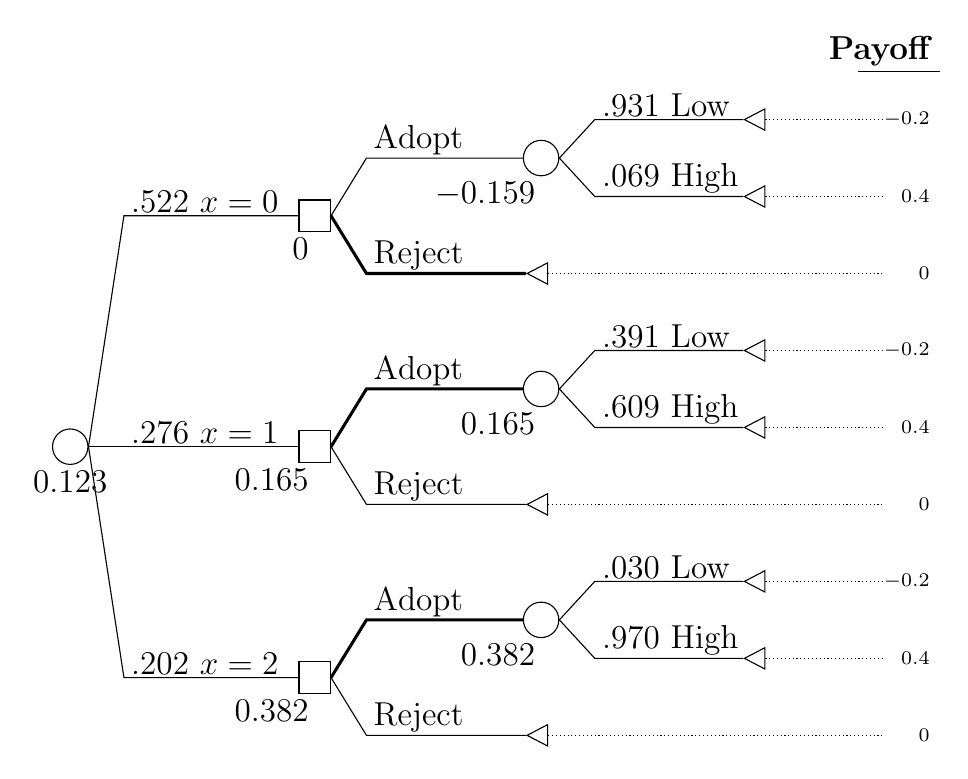
\begin{tikzpicture}[x=1.15cm,y=1.15cm]
\node[chance] (root) at (0,-3.6125) {};
\node[nval] at (root.south) {$0.123$};
\payoffheader{0.75}
\sigblock{root}{0}{.522\ $x=0$}{.931}{.069}{$0$}{$-0.159$}{plain}{opt}
\sigblock{root}{-2.55}{.276\ $x=1$}{.391}{.609}{$0.165$}{$0.165$}{opt}{plain}
\sigblock{root}{-5.1}{.202\ $x=2$}{.030}{.970}{$0.382$}{$0.382$}{opt}{plain}
\end{tikzpicture}}
\caption{Experiment $F$.}
\end{subfigure}
\hfill
\begin{subfigure}[t]{0.45\textwidth}\centering
\resizebox{\linewidth}{!}{%
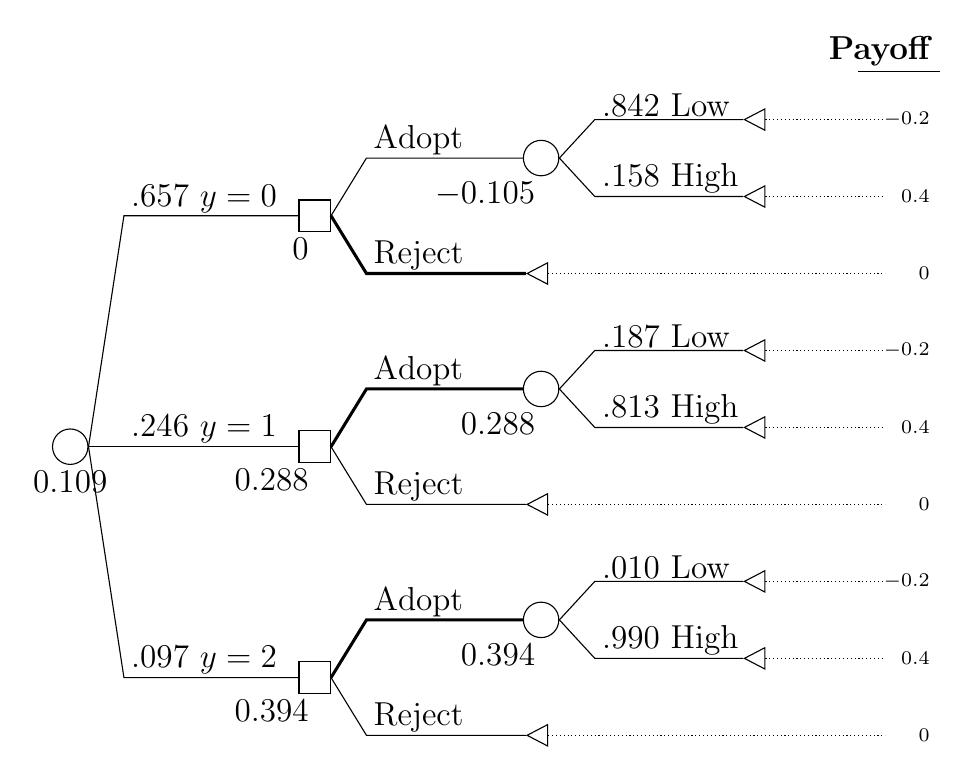
\begin{tikzpicture}[x=1.15cm,y=1.15cm]
\node[chance] (root) at (0,-3.6125) {};
\node[nval] at (root.south) {$0.109$};
\payoffheader{0.75}
\sigblock{root}{0}{.657\ $y=0$}{.842}{.158}{$0$}{$-0.105$}{plain}{opt}
\sigblock{root}{-2.55}{.246\ $y=1$}{.187}{.813}{$0.288$}{$0.288$}{opt}{plain}
\sigblock{root}{-5.1}{.097\ $y=2$}{.010}{.990}{$0.394$}{$0.394$}{opt}{plain}
\end{tikzpicture}}
\caption{Experiment $G$.}
\end{subfigure}
\caption{Decision trees for the two-state technology adoption example ($\theta\in\{0.1,0.7\}$, prior on the high state $0.4$, adoption cost $0.3$). }
\end{figure}




\section{Preliminaries}


We study different information structures that provide signals about the underlying uncertain state. When can we say that one information source is better than the other? If the decision maker (DM) observes signals from information source $X$ instead of information source $Y$, when are they better off?

Let $\theta\in \Theta \subseteq \Re$ be the state of the world, for example, the value of a new technology in a technology adoption model or the state of a machine in a machine replacement model. The DM is uncertain about the state of the world, and their beliefs are described by a probability distribution. For ease of notation, we will assume that the DM's probability distribution is continuous and has a density $\pi$ over $\Theta$.


In each time period, the DM chooses whether to adopt the technology, reject it, or gather additional information. If the DM chooses to gather information about the state of the world, they pay $c$ in that period and observe a signal $x\in X$ drawn from a likelihood function $L(x|\theta)$.







\section{Normal likelihood}
Let $F(x|\mu, \sigma^2)$ be a Normal signal-generating process with mean $\mu$ and variance $\sigma^2$. This likelihood satisfies the MLR property. Suppose that we add a bias term that depends on the unknown mean $\mu$ and observe
\begin{equation}
    Y=X+d(\mu)+Z
\end{equation}
instead, where $d(\mu)$ is a decreasing function of $\mu$ and $Z$ is a normally distributed error term with mean 0 and variance $\nu^2$. Then, we have
\begin{equation}
    H(y|x, \mu, \nu^2)\sim N(x+d(\mu), \nu^2)
\end{equation}
This state-dependent garbling function is a conditional probability distribution that is LR-decreasing in $\mu$ because $d(\mu)$ is a decreasing function. For example, $d(\mu)=-\delta\frac{\mu}{\sigma}$.

Given the definition of the biased signal-generating process $\iY$, we have that
\begin{equation}
    G(y|\mu, \sigma^2, \nu^2)\sim N(\mu+d(\mu), \sigma^2+\nu^2)
\end{equation}
which also satisfies the MLR property provided that $\mu+d(\mu)$ is increasing. For example, this would hold if we have $d(\mu)=-\delta\frac{\mu}{\sigma}$ for $\delta\leq \sigma$.

Then, likelihood $F$ ``LR-MQG dominates" likelihood $G$. Since  both likelihoods have the MLR property, we can conclude that a monotonic DP has a higher value function with likelihood $F$.

If $d(\mu)$ is constant, we would have that  $F$ ``Blackwell-dominates"  $G$.

% A simulated example yields the likelihoods in \Cref{fig:NormEx}.
% \begin{figure}[h!]
%     \centering
%     \includegraphics[width=0.8\linewidth]{FigNormEx.JPG}
%     \caption{Simulated Normal likelihoods $F$ and $G$}
%     \label{fig:NormEx}
% \end{figure}

\section{Poisson likelihood}

Let $F(x|\lambda)$ be a Poisson distribution with rate $\lambda$, which has the MLR property in $\lambda$. Suppose, instead, each arrival in this process is observed with probability $d(\lambda)$. Then, the garbling distribution, $H(y|x, d(\lambda))$ is a Binomial distribution with the number of trials equal to $x$ and the success probability equal to $d(\lambda)$. This garbling distribution is LR-decreasing in $\lambda$ if $d(\lambda)$ is decreasing. We will show that after garbling, the resulting distribution is a Poisson distribution with rate $d(\lambda)\lambda$.
\begin{align}
    g(y|\lambda)&=\sum_{x=y}^\infty h(y|x, \lambda) f(x|\lambda)\, dx\\
    &=\sum_{x=y}^\infty{x \choose y} [d(\lambda)]^y [1-d(\lambda)]^{x-y}\frac{e^{-\lambda}\lambda^x}{x!}\\
    &=\frac{e^{-\lambda}[d(\lambda)]^y}{y!}\sum_{x=y}^\infty \frac{\lambda^x[1-d(\lambda)]^{x-y}}{(x-y)!}\\
    &=\frac{e^{-\lambda}[d(\lambda)]^y}{y!}\sum_{z=0}^\infty \frac{\lambda^{z+y}[1-d(\lambda)]^{z}}{z!}\\
    &=\frac{e^{-\lambda}[d(\lambda)]^y\lambda^y}{y!}\sum_{z=0}^\infty \lambda^{-y}\lambda^{z+y}\frac{[1-d(\lambda)]^{z}}{z!} \\
    &=\frac{e^{-\lambda}[d(\lambda)\lambda]^y}{y!}\sum_{z=0}^\infty \frac{\left(\lambda[1-d(\lambda)]\right)^{z}}{z!} \\
    &=\frac{e^{-\lambda}[d(\lambda)\lambda]^ye^{\lambda(1-d(\lambda))}}{y!} \\
     &=\frac{e^{-\lambda d(\lambda)}[d(\lambda)\lambda]^y}{y!}
\end{align}

The second equality follows from the definitions of binomial and Poisson distributions. The third equality follows because ${x \choose y}=\frac{x!}{(x-y)!y!}$. The fourth equality is taking $z=x-y$ and rewriting. The seventh equality follows because $\sum_{z=0}^\infty \frac{x^{z}}{z!}=e^x$.

The resulting Poisson distribution with rate $d(\lambda)\lambda$ has the MLR property if $d(\lambda)\lambda$ is increasing in $\lambda$.

\section{Uniform likelihood}
Let $F(x|\theta)$ be a uniform distribution between 0 and $\theta$, which has the MLR property in $\theta$. Suppose instead of observing $X$, we observe
\begin{equation}
  Y=d(\theta)X
\end{equation}
Then, $Y|\theta$ has a uniform distribution between 0 and $d(\theta)\theta$ that has the MLR property if  $d(\theta)\theta$ is increasing in $\theta$.

For this transformation, the garbling distribution is:
\begin{align}
    H(y|x,\theta)=\left\{ \begin{array}{cc}
        1 & \mbox{if } y=xd(\theta)\\
        0 &  \mbox{otherwise}
        \end{array}\right.
\end{align}
To see  $H(y|x,\theta)$ is LR-decreasing, if $d(\theta)$ is decreasing in $\theta$, consider the inequality
\begin{equation}
 H(y^2|x,\theta^2)H(y^1|x,\theta^1) \leq H(y^2|x,\theta^1)H(y^1|x,\theta^2)
\end{equation}
Suppose $y^1=x d(\theta^2)\leq y^2=x d(\theta^1)$, then, the inequality above is satisfied because $0\leq 1$. For any other selection of $y^1\leq y^2$, both sides of the inequality is equal to zero.

\emph{Note}: I think the above example would work for $Y=X+d(\theta)$. I tried more general garbling distributions,   $H(y|x,\theta)$, that are not deterministic. For example, we can observe $x$ or $x d(\theta) $with equal probability (does not satisfy LR-decreasing property) or $H(y|x,\theta)$ is uniform between $x$ and $x+d(\theta)$ (is LR-decreasing if $d(\theta)$ is decreasing but the marginal for $y|\theta$ is a trapezoidal distribution and not clear if it can be made to have the MLR property).


% References
\bibliographystyle{unsrtnat}
\bibliography{references}


\end{document} 